\section{Introduction}\label{sec:introduction}

\Ac{NGS} has seen vast improvements in cost and speed over the past several decades, as described by \citeauthor{Schloss2008} \autocite{Schloss2008} and \citeauthor{Davey2011} \autocite{Davey2011}. \citeauthor{Behjati2013} \autocite{Behjati2013} write that \enquote{using \acs{NGS} an entire human genome can be sequenced within a single day. In contrast, the previous Sanger sequencing technology, used to decipher the human genome, required over a decade to deliver the final draft.} 
This led to the introduction and increased usage of \ac{NGS} in medical diagnostics performed by the \acf{DoHG@MHH}, as seen in \cref{figure:sequenced_samples_and_cost}.

\begin{figure}[H]
    \centering
	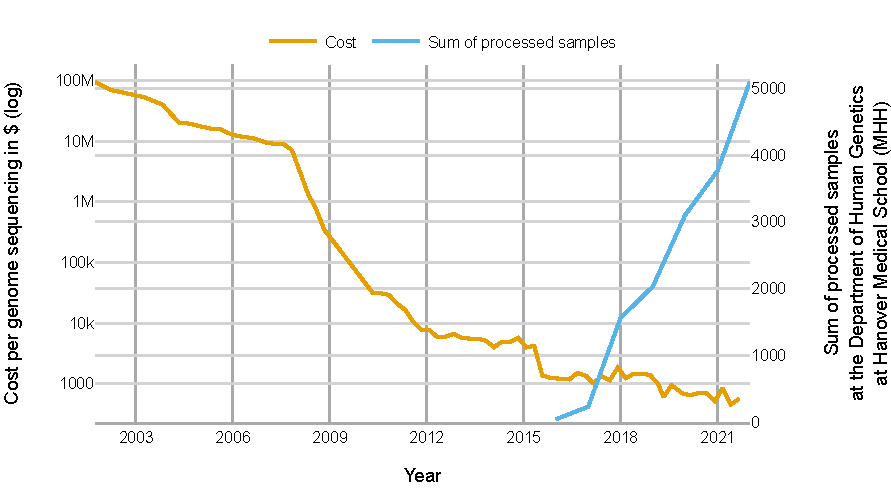
\includegraphics[width=\linewidth,height=\textheight,keepaspectratio]{sequenced_samples_and_cost}
	\caption[Comparison of cost per genome sequencing to the sum of processed samples at the \acs{DoHG@MHH}]{Comparison of cost per genome sequencing in U.S. dollar from \autocite{Wetterstrand2021} to the sum of processed samples at the \acl{DoHG@MHH} per year (see \cref{tab:sum_of_samples})}
	\label{figure:sequenced_samples_and_cost}
\end{figure}

Initially, whole-exome sequencing was introduced at the \ac{DoHG@MHH} in 2016. The exome covers nearly all the coding variation in an individual human genome and allows for a cost-effective analysis, as described in \autocite{Bamshad2011}. Starting in late 2021, following further cost reductions on the market, the genetic sequencing process at the \ac{DoHG@MHH} switched to whole-genome sequencing as recommended in \autocite{VanEl2013}. This covers all genetic data readable by the sequencing system, resulting in much more data being generated, as shown in \cref{figure:sequenced_samples_and_bases}.

\begin{figure}[H]
    \centering
    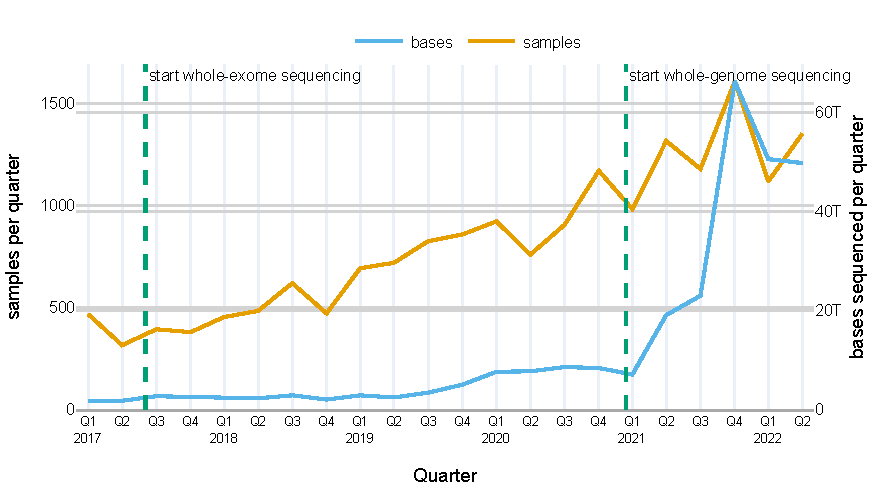
\includegraphics[width=\linewidth,height=\textheight,keepaspectratio]{sequenced_samples_and_bases}
    \caption[Number of samples and bases sequenced at the \acs{DoHG@MHH}]{Number of samples and bases sequenced at the \acl{DoHG@MHH} per year}
    \label{figure:sequenced_samples_and_bases}
\end{figure}

\citeauthor{Palladino2002} \autocite[p. 15]{Palladino2002}, \citeauthor{Patel2018} \autocite{Patel2018}, and \citeauthor{Caetano-Anolles2022} \autocite{Caetano-Anolles2022} define a reference genome as a representation of a species' complete DNA sequence used as a basis for comparisons with other genomic sequences. A reference genome serves as a standard by which variations in the genomes of individuals or populations of the same species can be characterized. There are several high-quality reference genomes available for numerous species, including humans (by the \textit{Human Genome Project} described in \autocite{Collins2003}), mice (e.g., \autocite{Lilue2018}), and many crops (see \autocite{Morrell2012}). These reference genomes are the result of extensive research efforts that involve the collection and analysis of DNA from multiple individuals and the integration of data from a variety of sources.

The data analysis pipeline and associated diagnostic tools at the \ac{DoHG@MHH} are currently based on the reference genome \textit{GRCh37} (\ac{UCSC} title: \textit{hg19}) released in 2009 (see \autocite{NLM2009}). It is used to align and sort the data fragments generated by the sequencing-by-synthesis technique used by the \ac{DoHG@MHH}'s \textit{NovaSeq 6000} \autocite{IlluminaInc.2022a} system by \textit{Illumina, Inc.} into a single sequence, a process described in \autocites{Holt2008}{Li2008}{Fuller2009} and usually called \textit{mapping}. In this context, a reference genome can provide a foundation for understanding the genetic differences that underlie health, disease, and diversity. 

\subsection{Problem}\label{subsection:problem}
The \ac{DoHG@MHH} uses the \textit{\acf{megSAP}} (\url{https://github.com/imgag/megSAP}) developed by the Institute of Medical Genetics and Applied Genomics at University Hospital and Faculty of Medicine T\"ubingen as its data analysis pipeline. In November 2021, the \textit{\ac{megSAP}} project switched to a newer reference genome, \textit{GRCh38} (\ac{UCSC} title: \textit{hg38}) (see \autocites{NLM2013}{Sturm2021}). The old version of the pipeline has been discontinued. In order not to fall behind, the \ac{DoHG@MHH} wants to upgrade to the newer pipeline version as soon as possible. But switching the reference genome is not a drop-in replacement. In addition to possible compatibility issues with external databases used by biologists and medical geneticists in the diagnostic process, several local configurations and, more importantly, all self-produced reference data, needs to be adopted or reprocessed. This raises a couple of problems to be solved:
\begin{description}
    \item[Processing capacity] The processing pipeline runs mainly on the \ac{MHH}'s \ac{HPC} cluster. There, the \ac{DoHG@MHH} has 17 nodes with a total of 656 CPU cores and \SI{5.106}{\tera\byte} RAM available. The \textit{NovaSeq 6000} handles up to \SI{48}{samples} in one run. Processing these uses all that capacity for \qtyrange{20}{24}{\hour} while being able to process 24 samples in parallel. No reprocessing can be done simultaneously, as diagnostic for current patients is time-sensitive and therefore has a higher priority. Investing in additional capacity in the short term is not feasible in the public service domain.
    
    \item[Storage capacity] At the \ac{DoHG@MHH}, sequencing data is stored in the BAM file format (see \autocite{Li2009}). Including analysis results, each sample takes approximately \SI{100}{\giga\byte} in size (compressed) for whole-genome data and \SI{10}{\giga\byte} for whole-exome data. About half of this are the BAM files that are backed up to tape storage after a successful run of the data analysis pipeline. All previously generated data has to be retrieved from tape storage for reprocessing. Roughly \num{1544} genome samples (see \cref{appendix:extrapolation}) are estimated to be present when the analytic pipeline is scheduled to migrate to \textit{GRCh38} in April 2023. Thus, about \(1544\text{ samples}\times50\text{ \unit{\giga\byte}}=77.2\text{ \unit{\tera\byte}}\) of storage is needed for the genome data alone. Currently, all storage provided to the \ac{DoHG@MHH} by the \ac{MHH} (\SI{95}{\tera\byte}) is in use. The remaining \SI{10}{\tera\byte} of space is reserved and needed for temporary file duplication while running the analytic pipeline.
    
    \item[Internet bandwith] Former undocumented tests with cloud infrastructure exposed another bottleneck: The \ac{MHH}  has imposed a restriction of a maximum of \unit{\mega\bit\per\second} of bandwidth (synchronously) for the \ac{DoHG@MHH}. Uninterrupted uploading to a cloud provider would take \(\frac{77.2\text{ \unit{\tera\byte}}}{500\text{ \unit{\mega\bit\per\second}}}=14.3\text{ \unit{\day}}\) to complete alone.
    
    \item[Processing time] As mentioned before, \SI{48}{samples} are produced by one sequencing run of the \textit{NovaSeq 6000} simultaneously (see step \textit{sequencing} in \autoref{fig:flowchart_overview}). These are then processed in parallel with the sequential analysis pipeline according to the steps shown in \autoref{fig:flowchart_overview}. Reanalyzing has to start with the step \textit{mapping}. Beginning at this step, the remaining process takes 20-24 \unit{\hour} to complete. As described before, processing capacity is limited, so only a batch of 24 samples may be processed in parallel. With ideal conditions (no delay between pipeline runs, exclusive usage of processing resources) this would result in a total reanalyzing time of roughly \(\frac{1544\text{ samples}}{24\text{ per batch}}\times22\text{ \unit{\hour}}\approx59\text{ \unit{\day}}\) for the whole-genome data.
    
    \item[Architecture] In its current state, \textit{\ac{megSAP}}, which is written in \textit{PHP}, is triggered by shell scripts. These scripts are written by researchers (biologists, biochemists and clinical geneticists) of the \ac{DoHG@MHH} and follow no particular design rules. There is no monitoring system in place, the current state of a pipeline run can only be interpreted by looking at the files found in the working directory and the list of running processes. Performance reporting can only be done by manually analyzing a log file with minimal information. The pipeline is executed in \ac{MHH}'s \ac{HPC} cluster using \textit{\ac{SLURM}}. About \SI{5}{\percent} of the processes fail with errors unknown to the users and have to be restarted manually (often after hours), which resolves the problem in almost all cases.
\end{description}

\begin{figure}[H]
    \centering
	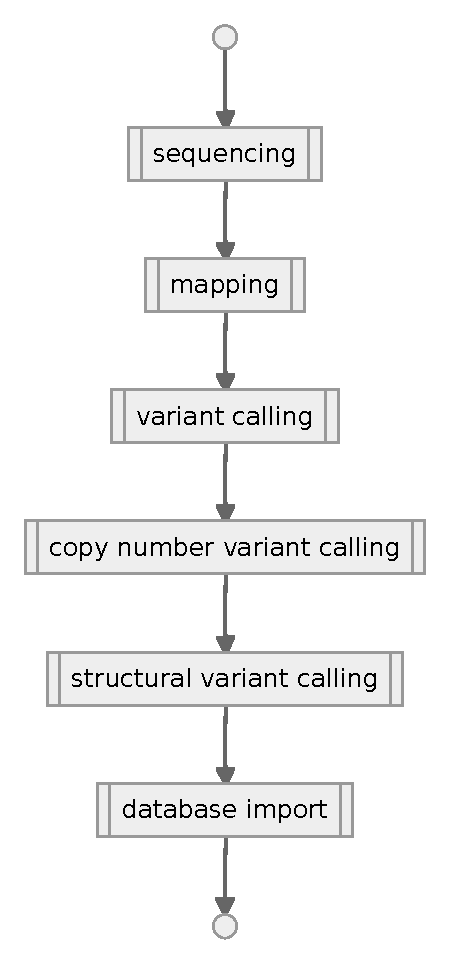
\includegraphics[scale=0.8]{flowcharts/overview}
	\caption[Overview of the genetic sequencing and analyzation process]{Overview of the genetic sequencing and analyzation process}
	\label{fig:flowchart_overview}
\end{figure}

\subsection{Goals}\label{subsection:goals}
The main objective to support the transition to a new reference genome is optimizing the analysis pipeline. Reanalysis must be performed as quickly as possible to allow the \ac{DoHG@MHH} to switch to \textit{GRCh38} as soon as possible. Two main ideas are explored, as described in the following subsections.

\subsubsection{Professionalization of Pipeline Utilization}
The current pipeline has been found to suffer from numerous issues related to a lack of computer science expertise among the scientists responsible for its implementation. Due to limited time dedication to this task, it has been proposed that adoption of a \ac{SWfMS} would provide a solution to the challenges outlined previously. This approach would promote reproducibility of results, facilitate automatic retries, and enable more transparent error reporting. In support of this proposal, initial research has identified potential \ac{SWfMS} candidates, including \textit{Nextflow} (\url{https://www.nextflow.io/}) and \textit{Snakemake} (\url{https://snakemake.github.io/}), that will be evaluated, among others, based on their suitability. It is important to consider the accessibility and usability of the \ac{SWfMS}, as the pipeline is expected to be used and maintained by biologists and medical staff in the future.

\subsubsection{Usage of Cloud Services}
The utilization of cloud computing for processing large data sets is a compelling proposition. Among the various cloud providers, \textit{\ac{AWS}} offers specialized \textit{F1} instances through their \textit{\ac{EC2}} service with \ac{FPGA} support, as documented in \autocite{AmazonWebServices2022}. Additionally, \ac{AWS} provides official pre-installed \textit{DRAGEN} software, shown in \autocite{AmazonWebServices2023a}. Nevertheless, the main challenge in implementing such a solution is the limited bandwidth, as outlined in \autoref{subsection:problem}. Despite this challenge, solutions such as \textit{\ac{AWS} Snowball} (\url{https://aws.amazon.com/snowball/}, \autocite{AmazonWebServices2022b}) may offer a viable solution, and will be assessed.

However, it is important to consider the potential cost associated with the use of cloud services, as it entails additional expenses for the \ac{DoHG@MHH}. Therefore, it is necessary to carefully estimate the cost of such an endeavor.